\documentclass[a4paper,11pt,DIV=calc,tablecaptionabove,headinclude,twoside]{article}
\usepackage[utf8]{inputenc}
\usepackage{ngerman}
\usepackage{caption}
\usepackage{amsmath}
\usepackage{amssymb}
\usepackage{array}
\usepackage{booktabs}
\usepackage{fancyhdr}                   %% Seite, Kopf- und Fußzeile anpassen (siehe \usepackage{geometry})
\usepackage{flafter}                    %% verhindert dass Abbildungen vor Überschrift kommen
\usepackage{float}
\usepackage{etoolbox}
\usepackage[pdfpagelabels=true]{hyperref}
\usepackage{geometry}                   %% Seitenmaße verändern (siehe \usepackage{fancyhdr}) !!! Das Paket IMMER nach hyperref einbinden!!!
\usepackage{graphicx}                   %% Einbinden von Bildern mit \includegraphics[]{×}
\usepackage{tabularx}
\usepackage{eurosym}
\geometry{a4paper, top=27mm, left=30mm, right=20mm, bottom=30mm, headsep=10mm, footskip=10mm}
\usepackage[decimalsymbol=comma, binary-units=true, loctolang={DE:ngerman}]{siunitx}
% --------------------------- BibTeX ---------------------------------------
\usepackage[square]{natbib}                 
\bibliographystyle{natdin}           %% Referenzierung: Autor und Jahreszahl
%\bibliographystyle{lex2018}


% Title Page
\title{Experimentplanung LEX 2018}%:\\Messseeelefantenantennenbenennungsverfahren}
\author{Theresa Lang, Laura Dietrich, Joscha Fregin, Simon Michel, Henning Dorff und Jakob Dörr}

\begin{document}
\maketitle



\section{Einleitung}
\subsection{Motivation}
%Warum ist das Thema interessant bzw. relevant? Warum lohnt es sich, sich mit dem Thema zu beschäftigen? (0.5--1 Seiten)\\\\
Die Grenzschicht ist der Bereich der Atmosphäre, der direkt vom Boden beeinflusst ist. Dazu zählen bespielsweise der Einfluss von Reibung am Erdboden, Strahlungsprozesse und der generelle Energieaustausch zwischen Boden und Atmosphäre. Die meisten für uns bedeutsamen Wetterparameter, wie bodennahe Temperatur und Wind, die relative Feuchte oder die Stabilität und Gewitterwahrscheinlichkeit hängen vom Zustand der Grenzschicht ab. Auch wichtige Wetterphänomene, wie die Nebelbildung oder die Land-Seewind Zirkulation finden hier statt.\\\\
Ein gutes Verständnis und eine präzise Modellierung der Grenzschicht ist nicht nur für eine gute Wettervorhersage unablässlich, sondern auch beim Bau großer Gebäude, beim Flugverkehr, der Ausbreitung von Schadstoffen oder für die Optimierung von Windkraftanlagen von Bedeutung. Hierfür sind gut aufgelöste in-situ Messungen der Grenzschicht nötig.\\\\
Im Rahmen der LEX bietet sich uns eine einzigartige Möglichkeit, den Aufbau der Grenzschicht in küstennahen Regionen besser zu verstehen, da wir kontinuierliche, zeitlich und vertikal hochaufgelöste in-situ Profilmessungen bis in 1000\,m Höhe durchführen können. Von einigen Parametern, wie der Temperatur oder der Feuchte gibt es nur wenige kontinuierliche Profilmessungen in dieser Höhe. Durch unsere gute Auflösung selbst in höheren Bereichen der Grenzschicht erhoffen wir uns, die zeitliche Entwicklung der Grenzschicht im Messzeitraum besser zu verstehen und möglicherweise sogar neue Erkenntnisse aus diesen abzuleiten.

\subsection{Wissenschaftliche Ziele/Fragen}
%Jedes Ziel mit Bullet-Punkten kurz und prägnant definieren; ein bis zwei -- auch stichwortartige -- Sätze genügen; nach Möglichkeit Hypothesen/Fragen formulieren, die im Experiment überprüft/beantwortet werden sollen. (wenige, 1 bis 5 Ziele)
Folgende Fragen und Ziele erhoffen wir uns im Rahmen unseres Experiments zu beantworten und zu erreichen:
\begin{itemize}
\item Entwicklung und Test einer eigenen Messhardware zur Profilmessung von
    Temperatur, Feuchte und Druck
\item Wie entwickelt sich die morgentliche küstennahe Grenzschicht? Auf welchen Zeitskalen spielt sich diese Entwicklung ab?
\item Wie beeinflusst die Anströmrichtung die Profile? Ist ein
    Landseewind erkennbar?
\end{itemize}

\section{Stand der Forschung}
%Was ist zum Thema bekannt? Welche Vorarbeiten (Paper, alte LEX-Berichte usw.) gibt es, an die angeknüpft werden kann?\\
Während des Experiments wird versucht, den Übergang zwischen nächtlichem und konvektivem Regime sowie Land- und Seewindregime am speziellen Fall einer küstennahen Grenzschicht zu untersuchen. \\\\
Über See unterliegen die Grenzschichtparameter nur geringen Schwankungen, da die Meeresoberflächentemperatur wenig variiert. Über Land hingegen kann sich die Grenzschicht auch auf kurzen Zeitskalen stark verändern und zeigt einen ausgeprägten Tagesgang. Die typische zeitliche Entwicklung der Grenzschicht bei einer sommerlichen Hochdruckwetterlage wird beispielsweise in \cite{stull1988introduction} beschrieben: Nachts schließt sich oberhalb der Prandtl-Schicht, die sich etwa über die untersten 10\% der Grenzschichtdicke erstreckt, die stabile nächtliche Grenzschicht an, die im Laufe der Nacht langsam anwächst. Darüber befindet sich die sogenannte „residual-layer“, bei der es sich um ein Überbleibsel der Mischungsschicht vom Vortag handelt. Nach Sonnenaufgang kommt es zu einem schnellen Zerfall der nächtlichen Grenzschicht und eine konvektive Mischungsschicht entwickelt sich oberhalb der Prandtl-Schicht. \\\\
%Übergang Land-/Seegrenzschicht (Henning)\\ % nur allgemeine Beschreibung
Dieser Tagesgang stellt sich unter idealisierten Verhältnissen ein und wird beispielsweise in Küstenregionen durch die Land-See-Zirkulation überlagert. Wegen der unterschiedlichen Wärmekapazitäten und der differentiellen Erwärmung von Land und Meeresoberfläche entsteht ein horizontaler Druckgradient zwischen beiden Oberflächen. Die tagsüber über dem erwärmten Land aufsteigenden Luftmassen erzeugen einen bodennah erniedrigten Luftdruck gegenüber der bodennahen Luft über dem Meer.  
Aus diesem Luftdruckgefälle stellt sich eine landeinwärts gerichtete Ausgleichströmung ein. Somit wird kühlere und feuchtere Seeluft advehiert. In der Folge dreht sich diese Zirkulation zum Nachmittag wegen der erniedrigten solaren Einstrahlung um. Somit wird auch die Küstengrenzschicht über Land während des Seewindes durch die Grenzschicht des Meeres beeinflusst. Der Tagesgang bzw. das Anwachsen der neutralen Grenzschicht über Land wird dabei durch das bodennahe Einströmen der bodennahen kalten Luftmassen abgeschwächt. Wie eine bodennahe Kaltfront sorgt die Zirkulation dann für eine Stabilisierung der Grenzschicht. Die Messbarkeit dieses Phänomens gestaltet sich bei synoptischen Einflüssen aber schwierig, da die großskalige Advektion unter anderem bei Frontendurchzug den Prozess überlagert. Dementsprechend sind ruhige Wetterlagen für eine Nachweisbarkeit erforderlich \citep{Lange2004}.\\\\
\citet{jimenez2016morning} untersuchten den morgendlichen Übergang zwischen verschiedenen Grenzschichtregimes auf der Insel Mallorca mithilfe von Ballons und Drohnen. Der Übergang konnte nicht nur erfolgreich gemessen werden, sondern stimmte auch mit Modellsimulationen überein.\\\\ 
\citet{Li2015TetheredBB} nutzten einen am Boden befestigten Ballon um die Aerosolkonzentraion von Rußpartikeln in der atmosphärischen Grenzschicht bis zu einer Höhe von 1000\,m über Shanghai zu messen. Bei den Messungen wurde ein Ballon mit einer Größe von 1600\,m$^{3}$ verwendet da schwerere Instrumente genutzt wurden. Zusätzlich wurde ein Lidar zur Windmessung verwendet. Da der Versuchsaufbau von \citet{Li2015TetheredBB} ähnlich zu unserem Versuchsaufbau ist sind wir optimistisch auch erfolgreich die Grenzschicht zu vermessen.\\\\
Aufgrund ihrer Flexibilität und dem relativ niedrigen Anschaffungspreis werden
in den letzten Jahren immer häufiger Drohnen für Messungen in der atmosphärischen Grenzschicht verwendet. \citet{kunz2018cocap} haben zum Beispiel COCAP entwickelt, ein Gerät zur Messung von CO2, das spezialisiert ist, um mit Drohnen zu fliegen. Die Temperatur und Feuchtesensoren von COCAP werden dabei unter den Rotoren der Drohne befestigt, sodass sie durch die 
Zugluft der Rotoren belüftet werden. Bei den Drohnenmessungen  der morgentlichen Grenzschicht auf Mallorca von \citet{jimenez2016morning} ergab sich eine gute Übereinstimmung mit Wetterstationen, Ballonmessungen und mesoskaligen Modellen. Hierbei waren die Sensoren über den Rotoren
der Drohne befestigt. Zum Einfluss des Downwash-Effektes einer Drohne auf die Messungen gibt es bisher wenig Erkenntnisse. \citet{zhou2017small} befand nach Testmessungen den Einfluss für minimal.\\\\
Zur Messung von Temperatur, Feuchte und Druck soll ein BME280 Sensor verwendet werden. In \citet{otte2018cost} wurde dieser Sensor in einer Klimakammer getestet und kalibriert. Nach der Kalibrierung wichen die Messungen des BME280 von den Referenztemperaturen um weniger als 0.1\,K ab. Bei guter Belüftung wurde für den Sensor eine Zeitkonstante von ca. 1\,s gemessen. Auf Basis dieser Ergebnisse gehen wir davon aus, dass der Sensor für unser Experiment geeignet ist.  

\section{Messstrategie}
%Wie sieht die allgemeine Messstrategie aus? Welche Größen sollen z.~B. mit welcher zeitlichen Auflösung gemessen werden, um die wissenschaftliche Fragestellung beantworten zu können?

Im Rahmen des Experimentes soll untersucht werden, wie sich die Größen Temperatur, Feuchte und Druck in der Grenzschicht im Verlauf eines Tages entwickeln, wobei besonderer Fokus auf den Übergang zwischen nächtlicher und konvektiver Grenzschicht gelegt werden soll. Zusätzlich sollen Erkenntnisse darüber gewonnen werden, ob und wie die küstennahe Grenzschicht durch die unmittelbare Nähe zum Meer beeinflusst wird und wie sich unterschiedliche Anströmrichtungen auswirken. \\\\
Die Kombination von zwei Messstrategien soll dies ermöglichen: Zur Beobachtung der zeitlichen Entwicklung werden mithilfe eines Helikites täglich ab Sonnenaufgang bis zum Nachmittag die Größen Temperatur, Feuchte und Druck in 10 Messhöhen zwischen 50\,m und 1000\,m mit einer zeitlichen Auflösung von 1\,s gemessen. Zusätzlich ist geplant, ein Lidar in der Nähe des Helikites zu installieren, mit dem Vertikalprofile von Windgeschwindigkeit und -richtung in hoher zeitlicher Auflösung gemessen werden. % Welche Auflösung usw.?
Um den Einfluss des Meeres auf die küstennahe Grenzschicht zu verstehen, soll zusätzlich eine Drohne verwendet werden, mit der zwei mal täglich instantane Horizontalprofile der Messgrößen über Land und Meer in mindestens zwei Messhöhen zwischen dem Boden und 100\,m Höhe gewonnen werden.
\subsection{Experimenteller Aufbau}
\label{Aufbau}
%Welche Instrumente sollen wie (Messhöhe, Standortwahl, horizontale Abstände, ... ) aufgebaut werden? (nach Möglichkeit Skizzen und Pläne hinzufügen)

Um die beschriebene Messstrategie umsetzen zu können, werden Messinstrumente an einem Helikite und an einer Drohne befestigt. Der Helikite hat ein Volumen von 14\,$\text{m}^{3}$, eine Tragfähigkeit von 7\,kg bei Windstille  
und kann auf eine Höhe von bis zu 1000\,m steigen \citep{helikite}. Er wird auf dem Hubschrauberlandeplatz des Bundeswehrgeländes in Marienleuchte in ca. 80\,m Entfernung zur Küste (Abbildungen \ref{messwiese} und \ref{flugroute_oben}) fest am Boden verankert. Nur für diesen Standort wurde eine entsprechende Aufstiegsgenehmigung beantragt. An der Leine des Helikites werden insgesamt 10 Messinstrumente in unterschiedlichen Abständen befestigt (Abbildung \ref{helikite}). Geplante Messhöhen sind 50\,m, 100\,m, 150\,m, 200\,m, 260\,m, 330\,m, 400\,m, 600\,m, 800\,m und 1000\,m, sodass die Abstände im unteren Bereich der Grenzschicht enger liegen als im oberen. Diese Abstände werden womöglich nicht exakt einzuhalten sein, da an der Leine des Helikites in bestimmten Abständen zusätzliche Markierungen befestigt werden müssen, die der Sichtbarkeit dienen. Die tatsächlichen Messhöhen lassen sich dann anhand des gemessenen Drucks bestimmen.
\begin{figure}[t]
\centering
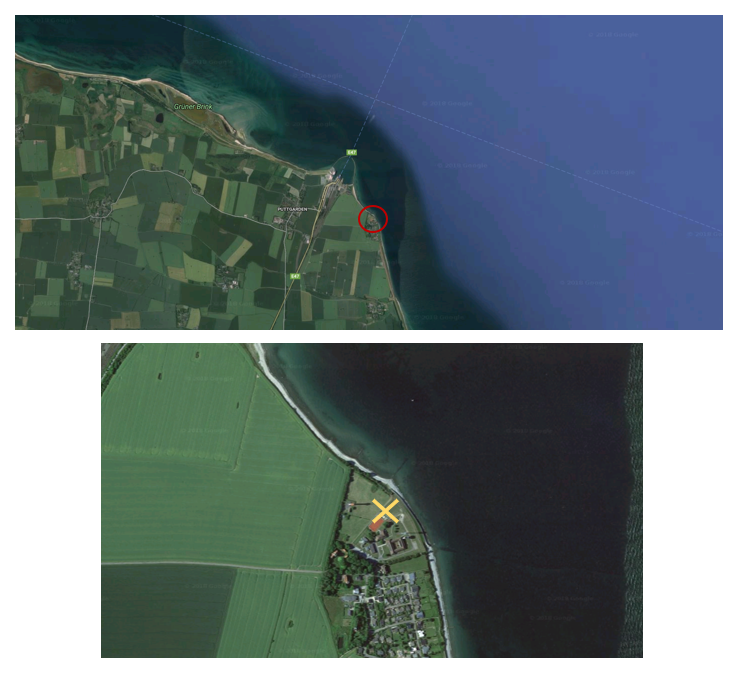
\includegraphics[width=0.8\textwidth]{Messwiese.png}
\captionsetup{width=11cm}
\caption{Lage des Messstandortes auf Fehmarn (oben) und Lage des Helikopterlandeplatzes auf dem Bundeswehrgelände (unten).}
\label{messwiese}
\end{figure}
\begin{figure}[t]
\centering
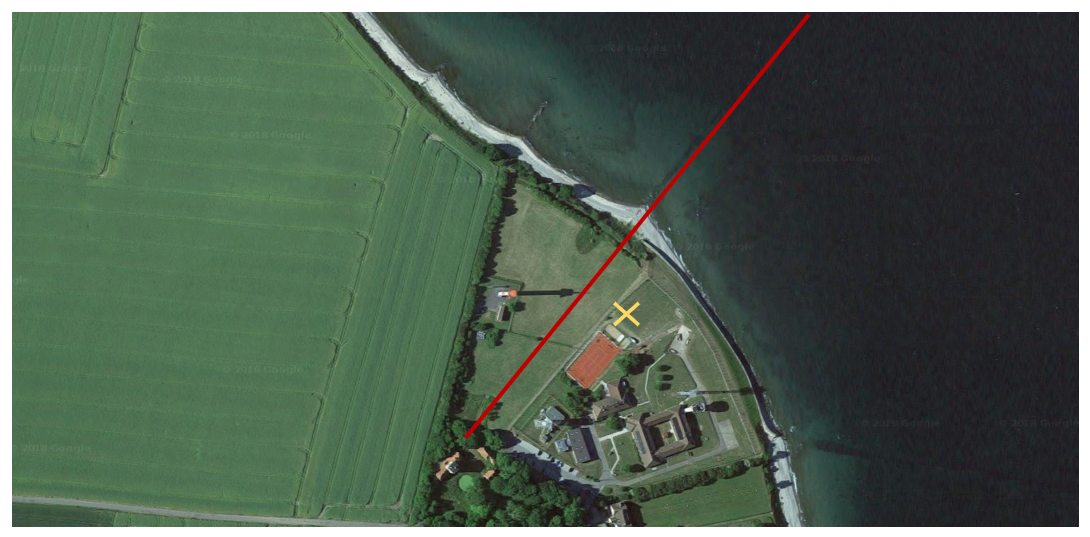
\includegraphics[width=0.7\textwidth]{Flugroute_oben.png}
\captionsetup{width=11cm}
\caption{Standort des Helikites (gelbes Kreuz) und geplante Flugroute der Drohne (rote Linie).}
\label{flugroute_oben}
\end{figure}
\begin{figure}[t]
\centering
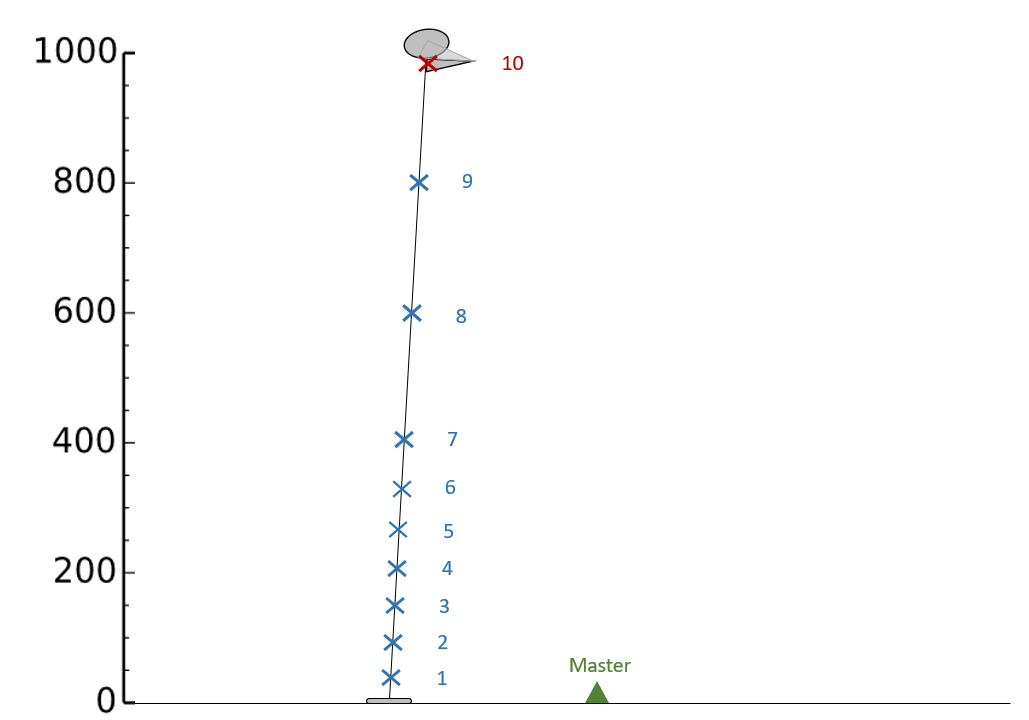
\includegraphics[width=0.7\textwidth]{Helikite.png}
\captionsetup{width=11cm}
\caption{Position der 9 Messinstrumente (blaue Kreuze) und dem Messgerät mit GPS-Modul (rotes Kreuz) an der Leine des Helikites und dem Master zum Empfangen der Daten am Boden (grünes Dreieck). }
\label{helikite}
\end{figure}
\\\\
Sollte ein Aufsteigen des Helikites aufgrund der Wetterbedingungen nicht möglich sein (siehe Abschnitte \ref{Bedingungen} und \ref{Risiken}), wird anstelle dessen bei niedrigen Windgeschwindigkeiten ein Fesselballon installiert, bei hohen Windgeschwindigkeiten ein Drachen. Die Messinstrumente werden in diesem Fall in äquidistanten Abständen bis zur maximal möglichen Messhöhe angebracht. \\\\
Alle Instrumente bestehen aus einem Arduino Board, einem BME280 Sensor zur Messung von Druck, Temperatur und relativer Feuchte und einem Long Range Wide Area (LoRa) Modul (Abbildung \ref{Slave}), das zur sofortigen Übermittlung der Daten zum sogenannten 'Master' am Boden dient (Abbildung \ref{Master}). Eine Übersicht über die technischen Daten des BME280 befindet sich in Abbildung \ref{BME_280}. Die Stromversorgung der Instrumente erfolgt mit Powerbanks mit einer Kapazität von 2000 mAh. Dies reicht auch bei maximalem Stromverbrauch der Messinstrumente weitaus mehr als einen Tag. Das oberste Instrument, das unmittelbar unterhalb des Ballons befestigt wird, verfügt zusätzlich über ein GPS Modul, sodass sich die Neigung der Leine aufgrund des Winds feststellen lässt. Die Instrumente werden in PVC-Rohren verpackt. Die einzelnen Bauteile werden dort so befestigt, dass sie nicht durch Stöße beschädigt werden können. Der Messsensor befindet sich außerhalb des Rohrs. So wird erreicht, dass der Sensor gut belüftet ist und verhindert, dass die Messungen durch ein strahlungsbedingtes Aufheizen oder Abwärme der anderen Komponenten innerhalb des Rohrs beeinflusst werden.\\\\
Jedes der Messgeräte inklusive Verpackung und Befestigungsvorrichtung wiegt ca. 200\,g, sodass das Gesamtgewicht deutlich unter der Nutzlast des Helikites liegt.\\\\
\begin{figure}[t]
	\centering
	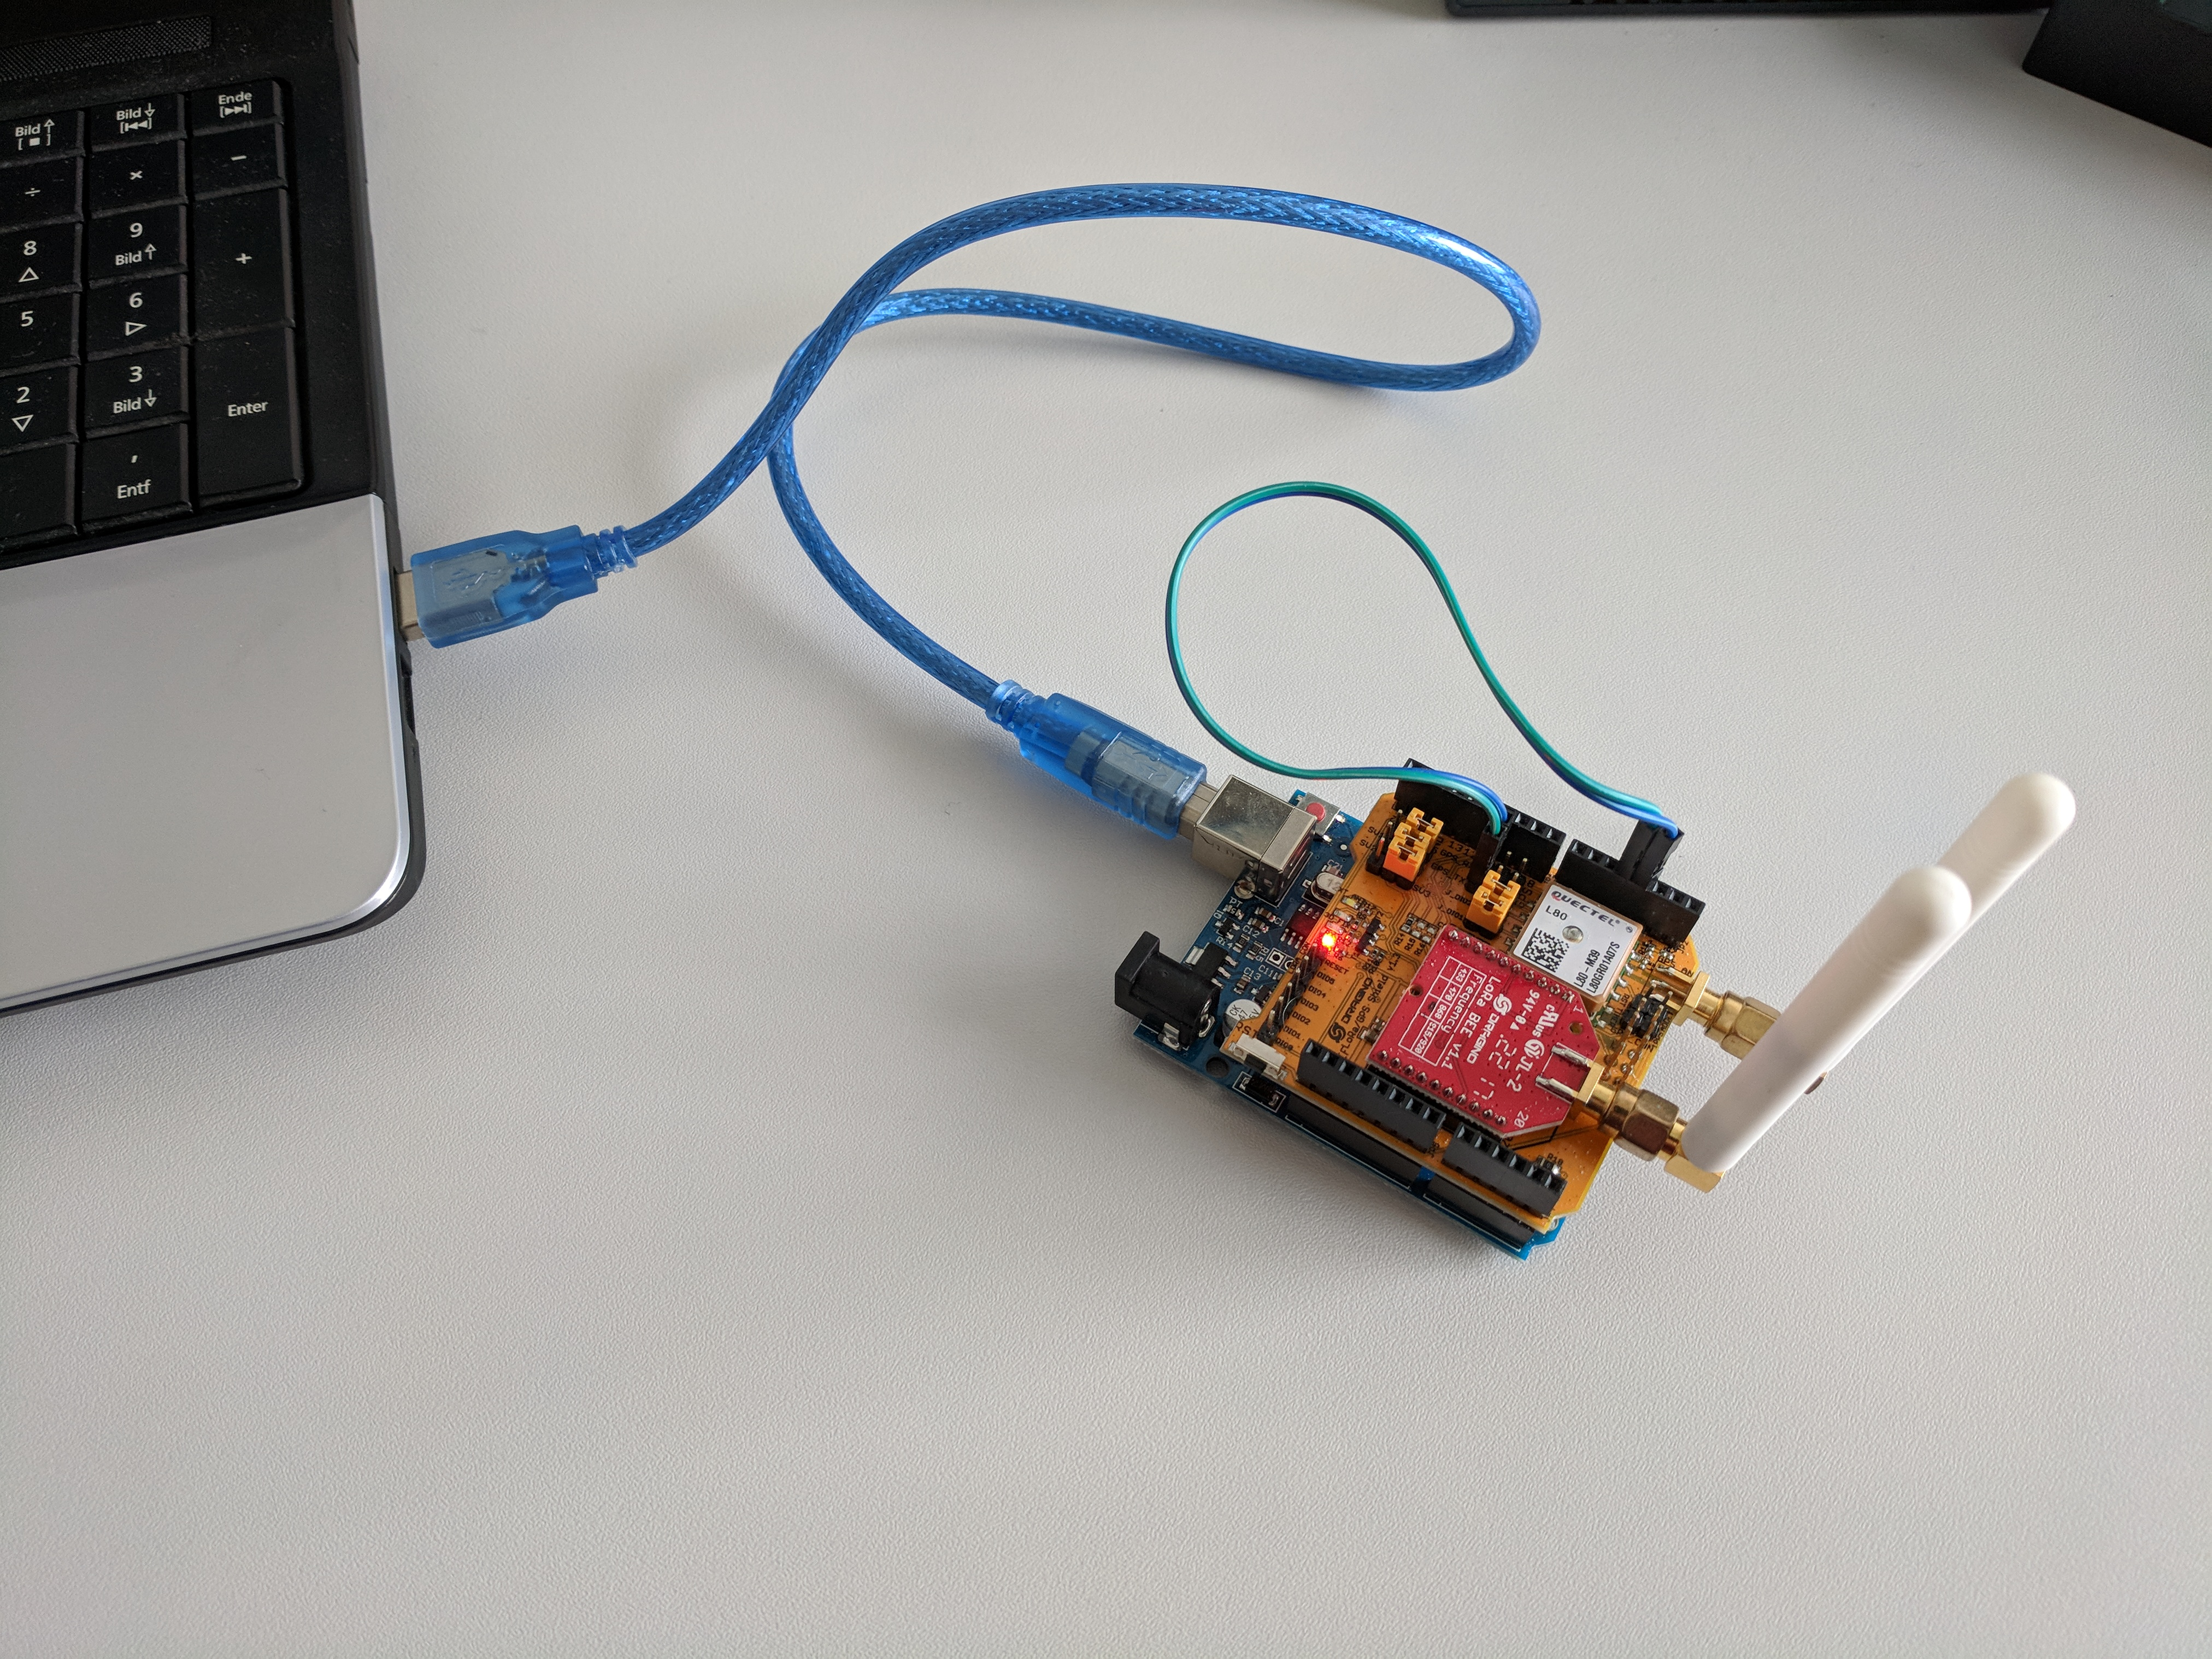
\includegraphics[width=0.7\textwidth]{Master.jpg}
	\captionsetup{width=11cm}
	\caption{Emfpangsstation 'Master' am Boden.}
	\label{Master}
\end{figure}
\begin{figure}[t]
	\centering
	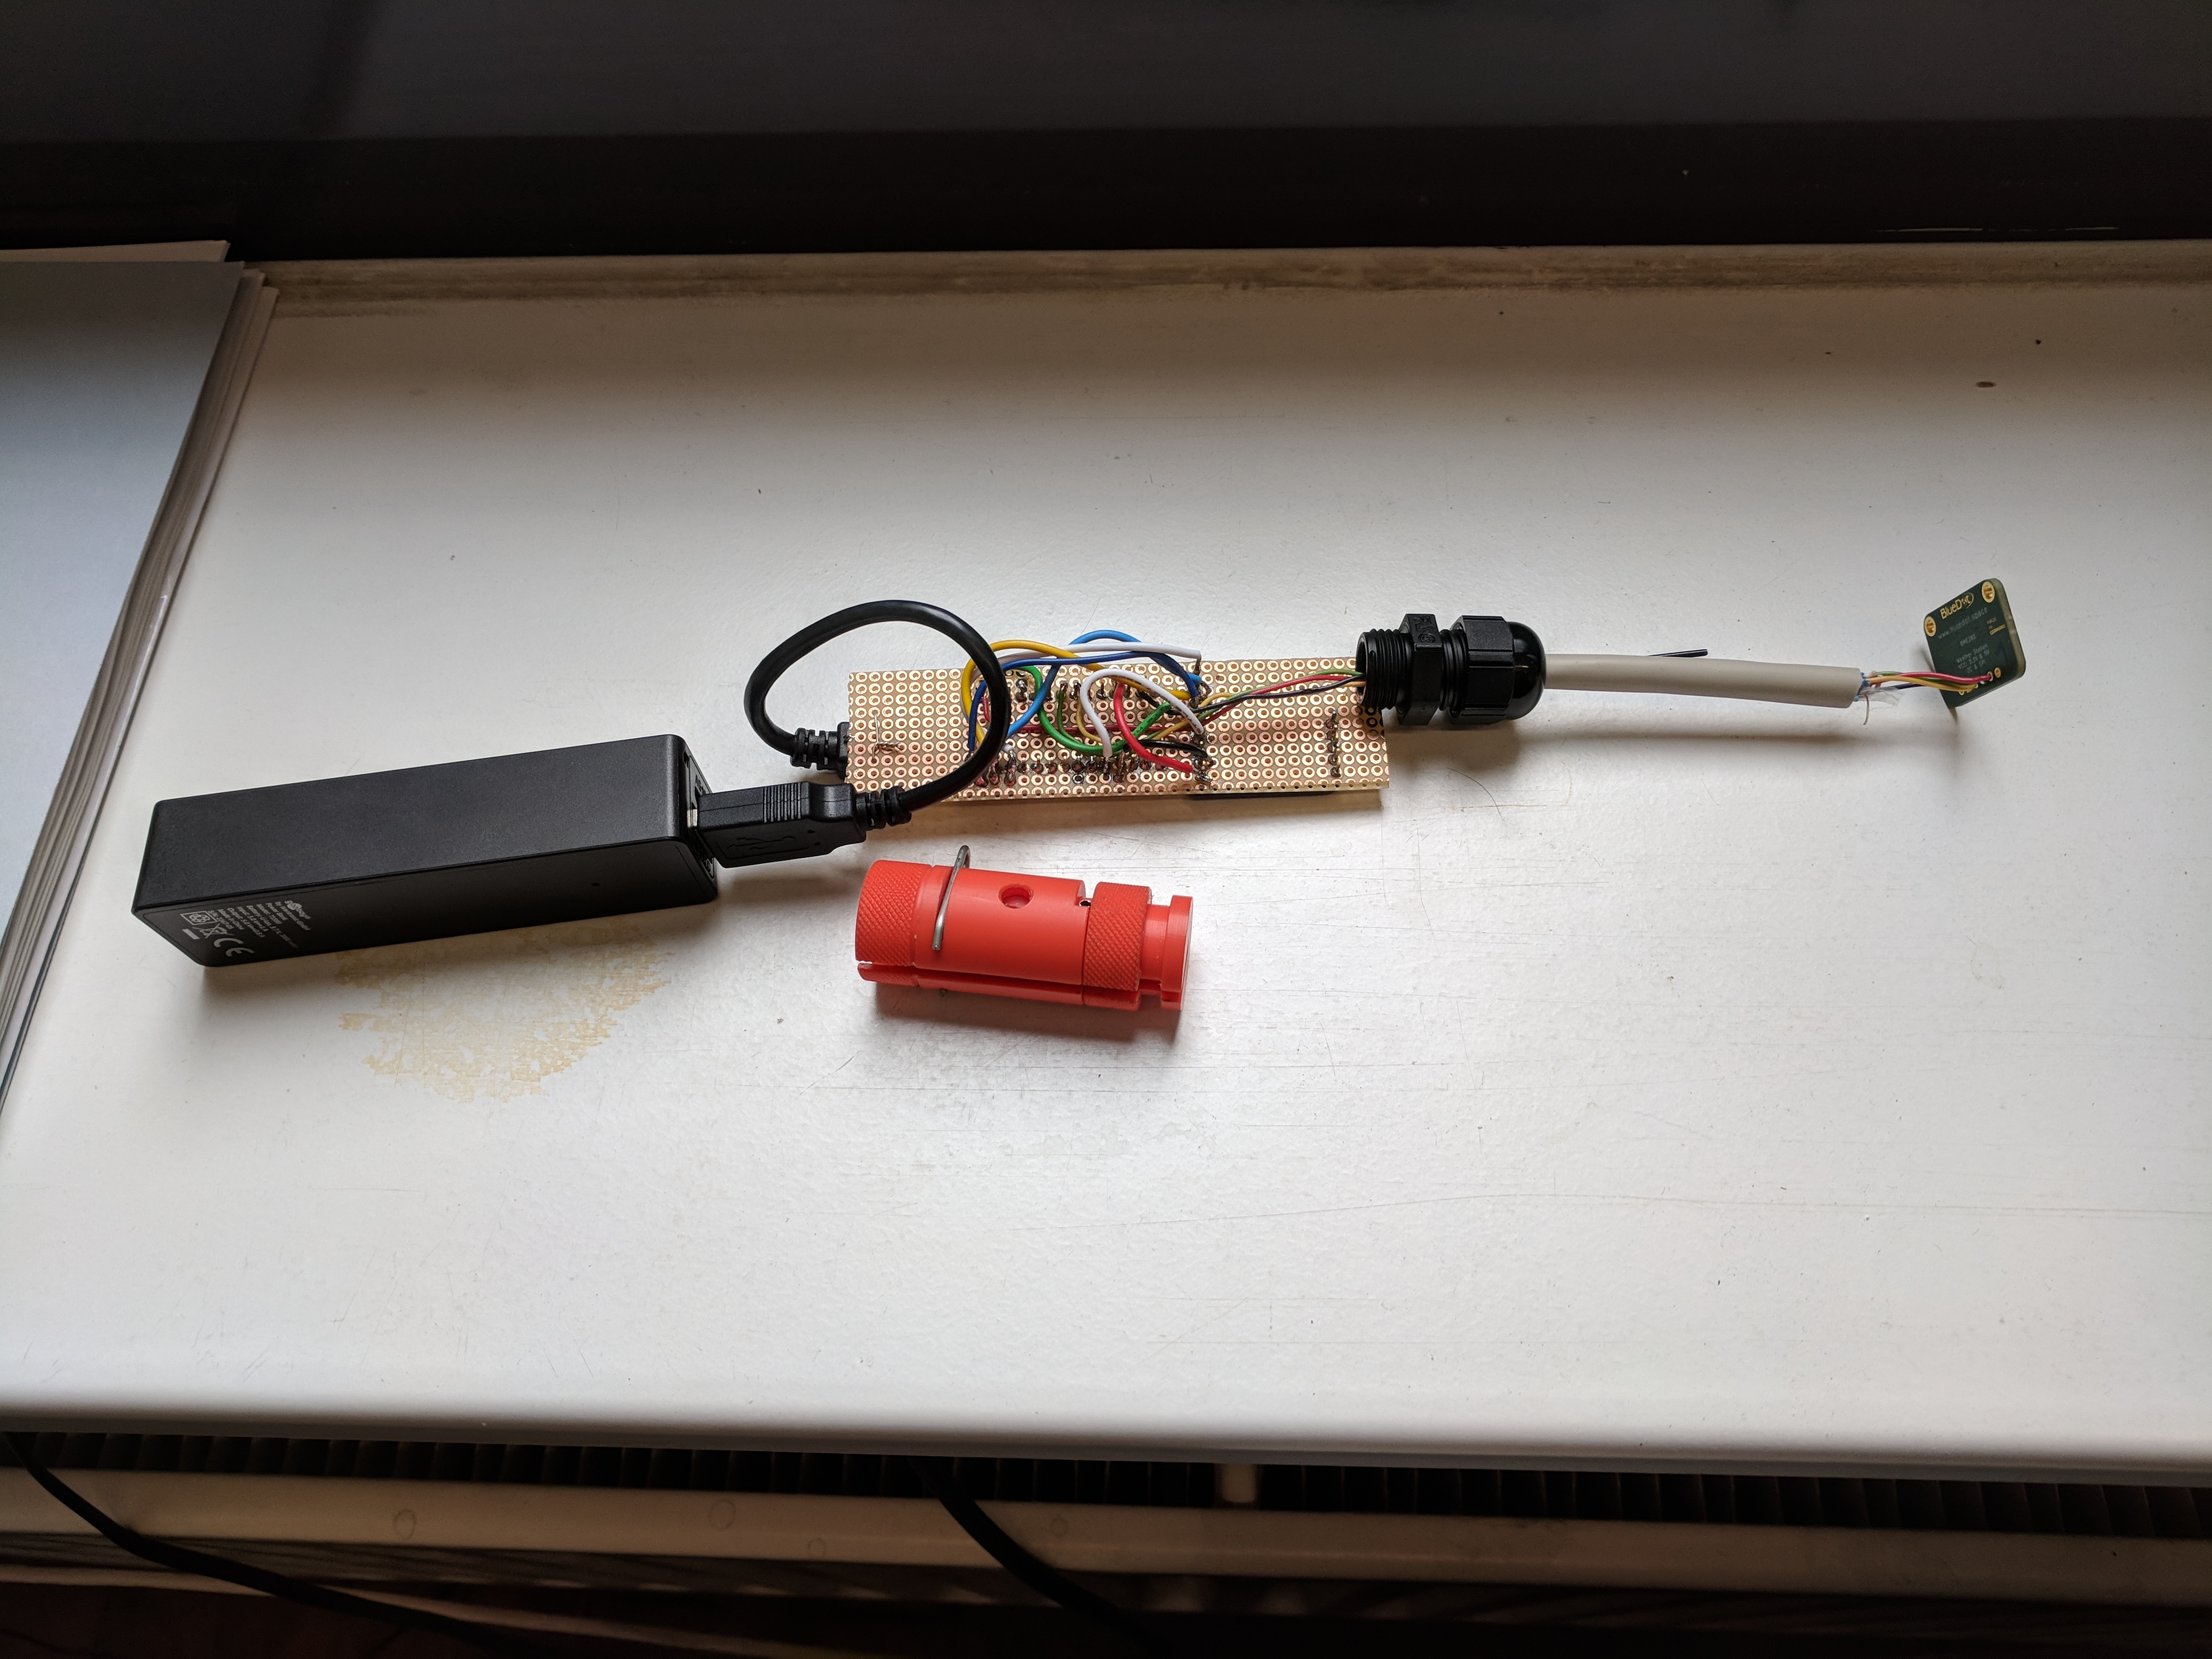
\includegraphics[width=0.7\textwidth]{Slave.jpg}
	\captionsetup{width=11cm}
	\caption{Aufbau eines Messinstruments ohne Verpackung. Links die Powerbank, in der Mitte die Leiterplatte mit Arduino Board und LoRa Modul auf der Rückseite und rechts der BME280 Sensor. Unten in Rot ein Teil der Vorrichtung zur Befestigung am Seil.}
	\label{Slave}
\end{figure}
Ein weiteres Messgerät gleicher Bauart (mit GPS Modul) wird direkt an der Unterseite einer Drohne des Typs DJI Phantom 2 befestigt. Diese hat eine Nutzlast von maximal 500\,g und eine Flugdauer von ca. 10 Minuten. Sie kann eine Maximalgeschwindigkeit von 15\,m/s erreichen, was somit gleichzeitig der maximalen Einsatzwindgeschwindigkeit entspricht. Das geplante Flugmuster der Drohne wird in Abschnitt \ref{sec:Durchfuehrung} beschrieben. \\\\
Ein Lidar der Firma METEK wird ebenfalls auf dem Gelände der Bundeswehr installiert. Genaue Angaben zu vertikaler und zeitlicher Auflösung können zum jetzigen Zeitpunkt noch nicht gemacht werden, da wir noch keine Informationen zum Lidar erhalten haben.  
\begin{figure}[b!]
\centering
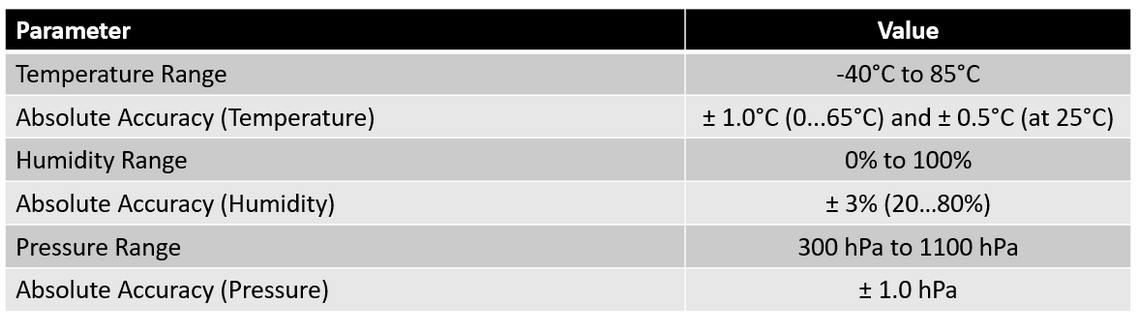
\includegraphics[width=\textwidth]{BME_280_technische_Daten.png}
\captionsetup{width=11cm}
\caption{Technische Daten des BME280 bluedot Sensors. Quelle: https://www.bluedot.space/sensor-boards/bme280/}
\label{BME_280}
\end{figure}

\subsection{Bedingungen/Erfordernisse}
\label{Bedingungen}
%Welche externen Bedingungen sind notwendig (Wetter)? Welche internen Erfordernisse sind notwendig (Betriebsmittel, Personal, externe Daten zur Durchführung usw.)? Sind Messdaten der anderen Gruppen erforderlich (Messstrategie absprechen)?

Folgende externe und interne Erfordernisse sind notwendig, um die geplanten Messungen erfolgreich durchführen zu können.

\subsubsection{Externe Bedingungen}

Die wichtigste externe Voraussetzung ist die Wetterlage, da die Messungen nicht bei Niederschlag durchgeführt werden können. Wie in Abschnitt \ref{Aufbau} beschrieben, ist der Sensor nicht wie der übrige Teil der Messgeräte durch eine Verpackung geschützt. Er sollte jedoch auf keinen Fall mit Wasser in Berührung kommen, um eine Beschädigung der Elektronik zu verhindern. Gleiches gilt auch für die Drohne. Auch bei hohem Niederschlagsrisiko kann das Experiment nicht durchgeführt werden. \\\\
Für die Messungen mit der Drohne spielt die Windgeschwindigkeit eine wichtige Rolle. Das verwendete Modell kann laut Hersteller bis zu einer maximalen Windgeschwindigkeit von 15\,m/s geflogen werden. Wir rechnen jedoch damit, dass es nur bis zu deutlich geringeren Windgeschwindigkeiten (ca. 5\,m/s) möglich ist, die Drohne mit ausreichender Sicherheit und Genauigkeit zu steuern. \\\\
Auch für den Helikite müssen bestimmte Windbedingungen vorherrschen. Genaue Angaben zu maximalen oder minimalen Windgeschwindigkeiten können noch nicht gemacht werden, wir gehen jedoch davon aus, dass der Helikite auch für hohe Windgeschwindigkeiten ausgelegt ist.

\subsubsection{Interne Bedingungen}

Um den Helikite wie geplant einsetzen zu dürfen, ist eine behördliche Genehmigung nötig. Eine solche Genehmigung wurde für einen Aufstiegszeitaum zwischen Sonnenaufgang und Sonnenuntergang und für eine maximal Aufstiegshöhe von 1000\,m bereits beantragt und genehmigt.\\\\
Sowohl die Drohne als auch die Messinstrumente werden über Akkus mit Strom versorgt, die zwischen den Messphasen geladen werden müssen. In der Nähe des Messstandortes müssen deshalb ausreichend USB-Ladekabel und Steckdosen vorhanden sein.\\\\
Es muss damit gerechnet werden, dass es bei den Messinstrumenten zu Ausfällen kommt. Es müssen deshalb ausreichend Ersatzteile und Werkzeuge bereit liegen, um kaputte Bauteile möglichst schnell ersetzen zu können. Die Software der Messgeräte kann in Form sogenannter Sketches nur über einen PC auf den Arduino aufgespielt werden, sodass auch PCs mit der benötigten Software vorhanden sein müssen.\\\\
Für den Helikite bzw. den Ballon wird ausreichend Helium benötigt. Zudem muss für die Winde des Helikites am Messstandort (Helikopterlandeplatz) eine Stromversorgung vorhanden sein.

\subsection{Durchführung}
\label{sec:Durchfuehrung}
%Beschreibung des regulären Messablaufs. Sind Intensivmessphasen geplant? Auf welche besonderen Ereignisse soll wie reagiert werden? 
%Wann werden zusätzliche Messungen (z.\,B. Radiosondenaufstiege) durchgeführt?

Der reguläre Messtag startet ca. 1 bis 2 Stunden vor Sonnenaufgang, der im zwölftägigen Zeitraum der Messkampagne zwischen 6:15 Uhr (28.08.2018) und 6:35 Uhr (08.09.2018) stattfindet. Der Helikite muss bis zum Sonnenaufgang vollständig aufgebaut sein. Am ersten Tag planen wir für den Aufbau des Helikites 2 Stunden ein und das gesamte Team ist anwesend. Je nachdem, wie lange der Aufbau dauert können Zeit und Personenanzahl an den Folgetagen angepasst werden. Nach einer Überprüfung der Wetterlage entscheidet das Team, ob ein Aufstieg möglich ist. Während des Aufbaus müssen die Messinstrumente an ihre Powerbanks angeschlossen werden und auf Funktionalität geprüft werden. Anschließend werden sie in den in Abschnitt \ref{Aufbau} genannten Abständen an der Leine des Helikites befestigt, während wir diesen aufsteigen lassen. \\\\
Sobald die Messinstrumente mit Strom versorgt sind, werden ihre Messdaten in sekündlichen Abständen an den Master am Boden gesendet. Neben den Messwerten wird auch eine individuelle Kennung verschickt, die es ermöglicht, die empfangenen Daten dem jeweiligen Messinstrument zuzuordnen. Der Master ist an einen PC angeschlossen, mit dem die empfangenen Daten direkt ausgelesen und abgespeichert werden können. Außerdem werden die Profile von Temperatur, Feuchte und Druck live geplottet. So kann auf interessante oder unerwartete Entwicklungen reagiert werden und eventuell zusätzliche Messungen mit der Drohne durchgeführt  werden.\\\\
Planmäßig sollen Messungen bis ca. 15 Uhr stattfinden, danach wird der Helikite abgebaut. Das Wetter wird jedoch während des gesamten Messzeitraums beobachtet und es wird sofort mit dem Abbau begonnen, sobald sich Niederschlag oder eingeschränkte Sichtverhältnisse ankündigen. Während die Leine eingeholt wird, werden die einzelnen Instrumente abgenommen, gesammelt und ihre Powerbanks anschließend aufgeladen. \\\\
Am ersten Tag soll zusätzlich ein Vergleichsprofil mit einer Radiosonde gemessen werden, um die Messhardware am Helikite zu testen. Bei Bedarf können die Radiosondenaufstiege auch an weiteren Tagen durchgeführt werden.\\\\
Zweimal täglich finden Messungen von Vertikal- und Horizontalprofilen mit der Drohne statt. Die erste Messung findet unmittelbar nach Sonnenaufgang statt, die zweite am frühen Nachmittag. Dadurch erhoffen wir uns, die Grenzschicht in möglichst verschiedenen Zuständen zu beobachten. Der Bereich, der mit der Drohne abgeflogen werden kann ist dadurch limitiert, dass laut Vorschrift maximal bis zu einer Höhe von 100\,m und nur auf Sicht geflogen werden darf. Zusätzlich hat die Drohne nur eine begrenzte Akkulaufzeit von ca. 10 Minuten. Abbildung \ref{flugroute} zeigt das geplante Flugmuster. Da die Messungen Erkenntnisse darüber liefern sollen, ob und wie die Nähe zum Meer die küstennahe Grenzschicht beeinflusst, sollen die Vertikal- und Horizontalprofile sowohl über Land als auch über Wasser aufgenommen werden. \\\\
Die Drohne wird in ausreichendem Abstand zum Helikite gestartet und auf eine Höhe von ca. 20\,m gebracht. Anschließend soll sie senkrecht zur Küstenlinie über die Küste hinaus und über das Meer fliegen. Die Flugrichtung wird beibehalten, bis die Drohne sich ca. 250\,m vor der Küste befindet, wenn das Sichtfeld diese Entfernung erlaubt. Bevor die Drohne zurück fliegt erfolgt ein Aufstieg auf ca. 100\,m. Sobald die Drohne ca. 250\,m landeinwärts zurück gelegt hat, erfolgt ein Absinken zurück auf ca. 20\,m und die Drohne fliegt zurück zum Ausgangspunkt. Ist die Akkuladung zu diesem Zeitpunkt noch ausreichend hoch, können evtl. weitere Profile geflogen werden. \\\\
Um die gemessenen Profile von Drohne und Helikite zu vergleichen, sollen an einem Messtag zusätzlich Vertikalprofile mit der Drohne nahe des Helikites geflogen werden. Wie bereits erwähnt, darf die Drohne dabei maximal bis zu einer Höhe von 100\,m geflogen werden. 

\begin{figure}[t]
\centering
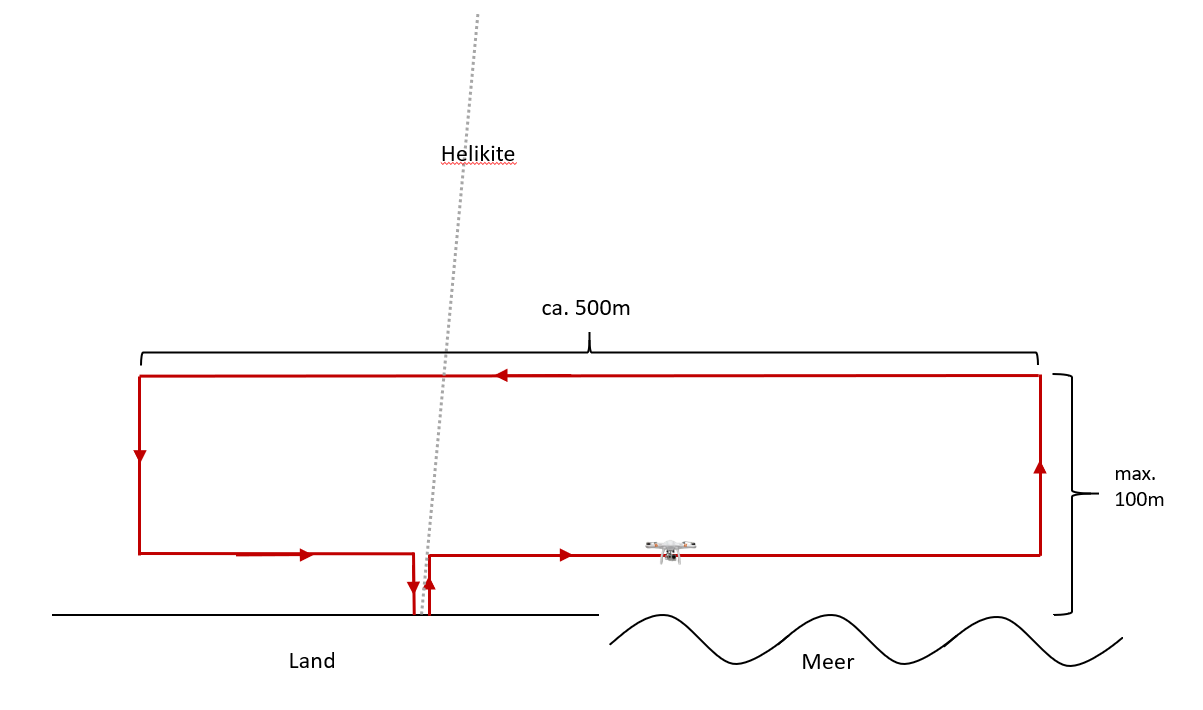
\includegraphics[width=0.9\textwidth]{Flugroute.png}
\captionsetup{width=11cm}
\caption{Geplante Flugroute der Drohne.}
\label{flugroute}
\end{figure}

\subsection{Auswertung}
%Wie sollen die Daten ausgewertet werden? Sind zusätzliche Daten (Satellitendaten, Modelldaten usw.) notwendig? Welche Grafiken oder Auswertungen sollen im Idealfall am Ende die wissenschaftlichen Fragen beantworten?\\

Alle im Experiment gesammelten Daten sollen mithilfe von Python ausgewertet werden. Die benötigten Programme zum Einlesen der Daten sollen bereits im Voraus entwickelt werden. \\\\
Zum Test der Messhardware (Helikite und Drohne) werden eines oder mehrere gemessene Profile mit gleichzeitigen Messungen einer Radiosonde verglichen. Zur Auswertung werden beide Profile in einem Plot dargestellt und vergleichend analysiert.\\\\
Zur Untersuchung der Entwicklung der Grenzschicht werden entweder gemessene Profile zu verschiedenen Zeiten in einen Plot Höhe gegen Temperatur/Feuchte/(Wind) aufgetragen oder eine komplette Messreihe in einen 2-D Konturplot Zeit-Höhe-Temperatur/Feuchte/Wind aufgetragen. So lassen sich Veränderungen der Grenzschicht sowie deren Zeitskalen analysieren, eventuelle Land-See-Wind-Regimes identifizieren und Veränderungen aufgrund eines Wechsels der Anströmrichtung erkennen.\\\\
Um die Profile der Drohne auszuwerten, werden in einem 3D-Plot zunächst die Flugrouten abgebildet und die gemessenen Temperaturen bzw. Feuchten farbig dargestellt. So lassen sich auch laterale Abweichungen vom Flugkurs feststellen. Zusätzlich werden die Flugrouten in Vertikal- und Horizontalprofile aufgeteilt. Vertikalprofile über Land und Meer werden in einem gemeinsamen Plot gegen die Höhe aufgetragen. Um den horizontalen Temperatur- und Feuchteverlauf darzustellen, werden die Messwerte in den Horizontalprofilen gegen den Abstand zum Startpunkt aufgetragen.    

\subsection{Risiken}
\label{Risiken}
%Woran könnten Teile des Experiments scheitern? Welche Alternativen gibt es in diesen Situationen? (für jedes Risiko einen Absatz)\\

Die Benutzung des Helikites bis in 1000\,m Höhe ist, wie oben beschrieben, an eine Wetterlage mit guter Sicht bis in 1000\,m ohne Sturm/stürmischen Wind gebunden. Falls diese Bedingungen nicht erfüllt werden, muss die Höhe des Helikites reduziert werden. Die Sensoren könnten dementsprechend in kürzerem Abstand aufgehangen werden und die Analyse der Grenzschicht bezieht sich nur auf diese Höhen. Im Falle eines vollständigen Ausfalls des Helikites kann auf Messungen mit einem Ballon und/oder Drachen zurückgegriffen werden. Diese fliegen nur bis etwa 100-200\,m. \\\\
Die entwickelten Sensoren sind nicht wasserfest und somit bei Niederschlag nicht einsetzbar. Bei 14 Tagen Regen am Stück würde das Experiment scheitern. In diesem Falle wäre eine Alternative, die Grenzschicht mit möglichst vielen Radiosondenaufstiegen zu untersuchen. \\\\
Auch die Messung der Windprofile mit dem Lidar hängt von der Wetterlage ab, da nur bis zur Wolkenunterkante gemessen werden kann. \\\\
Es besteht das Risiko, dass ein oder mehrere Sensoren ausfallen. Ein Ausfall des Masters am Boden wäre am schlimmsten, da dann keine Kommunikation mehr mit den anderen Sensoren möglich ist. Für den Fall von Sensorausfällen sind für beide Arduino-Typen mindestens ein Ersatz eingeplant. Auch für die LoRa Chips und für die BME280-Sensoren ist Ersatz vorhanden, der bei Ausfall zum Einsatz kommt.

\section{Kosten}
%Kosten für zusätzliches Material, Geräte, Betriebsmittel ...\\
%Die Materialkosten sind in Tabelle \ref{Tab:Kosten} aufgelistet.

Die Hauptkosten unseres Experiments entstehen durch die Bauteile der von uns selbst gebauten Messinstrumente. Deren Einzelpreis, Anzahl und Gesamtkosten sind in Tabelle \ref{Tab:Kosten} aufgeführt. Diese Kosten beziehen sich ausschließlich auf unser Teilprojekt der Lehrexkursion und beinhalten keine Kosten wie Personalkosten, Anreise, Verpflegung und Beschaffung des Helikites und anderer Instrumente. 

\begin{table}[h]
\caption{Auflistung der Materialkosten}
\begin{tabular}{|c|c|c|c|}
\hline
Bauteil & Preis (\euro) & Anzahl & Gesamtpreis (\euro) \\\hline \hline
RFM95W Lora Module 868MHz  & 7,00 & 12 & 84,00 \\\hline
Dragino Lora Shield 868MHz & 22,00 & 1 & 22,00 \\\hline
Arduino Nano & 7,00 & 11 & 77,00 \\\hline
Arduino Uno & 21,00 & 2 & 42,00 \\\hline
Dragino Lora/GPS Shield 868MHz & 35,00 & 1 & 35,00 \\\hline
Jumper Kabel male female & 0,20 & 100 & 20,00 \\\hline
Powerbank & 3,99 & 14 & 55,86 \\\hline
USB Kabel & 0,95 & 14 & 13,30 \\\hline
Bluedot BME280 Sensor & 20,00 & 18 & 360,00 \\\hline
Lochrasterplatinen Hartpapier 500x100mm H25PR500 & 6,45 & 3 & 19,35 \\\hline
SD-Karten Slot & 4,00 & 1 & 4,00 \\ \hline
GPS Chip & 15,00 & 1 & 15,00 \\\hline \hline
\textbf{Gesamtkosten} & & & \underline{\textbf{738,57}}  \\ \hline

\end{tabular}
\label{Tab:Kosten}
\end{table}

% BME-280
% Arduino Nano
% GPS chip
% Powerbank + Kabel
% evtl. SD-Kartenslot  
\newpage
\bibliography{Whitepaper}
\end{document}